%
% teil2.tex -- Beispiel-File für teil2 
%
% (c) 2020 Prof Dr Andreas Müller, Hochschule Rapperswil
%
% !TEX root = ../../buch.tex
% !TEX encoding = UTF-8
%
\section{Richardsons Ansatz \label{geostrophisch:section:richardsonAnsatz}}
\kopfrechts{Richardsons Ansatz}

Richardson wählte einen innovativen, aber im Grunde sehr einfachen Ansatz:  
Statt vereinfachter Modelle verwendete er ein vollständiges System bestehend aus vier Differentialgleichungen.
Die erste Gleichung:
\begin{equation}
	\frac{D\vec{v}}{Dt} + 2\vec{\Omega} \times \vec{v} = -\frac{1}{\rho}\nabla p + \vec{g} \\,
	\label{eq:navstok}
\end{equation}
ist eine Form der Navier-Stokes-Gleichung für rotierende Bezugssysteme.
$\frac{D\vec{v}}{Dt}$ entspricht der zeitlichen totalen Ableitung aller Geschwindigkeitskomponenten in Nord-, Ost- und Vertikalrichtungen.
Das grosse $D$ steht dabei für die totale Ableitung, dass bedeutet es wird die Änderung der Geschwindigkeit, wenn man sich mit der Luft bewegt, berechnet. 
Sie beschreibt also die Beschleunigung von Luftmassen und ausserdem werden darin die Coriolis-Kraft und der Druckgradient berücksichtigt.

Als nächstes verwendete er die Kontinuitätsgleichung:
\begin{equation}
	\frac{\partial \rho}{\partial t} + \nabla \cdot (\rho \vec{v}) = 0 \\,
	\label{eq:kont}
\end{equation}
welche die Massenerhaltung beschreibt, siehe dafür auch~\ref{buch:zusammenhang:erhaltungssatz:subsection:kontinuitaetsgleichung}.
Also in anderen Worten die Luft kann weder verschwinden noch aus dem Nichts auftauchen. 

Zudem brauchte er noch eine Gleichung, welche die Energie beschreibt, dazu diente 
\begin{equation}
	\frac{Ds}{Dt} = Q \\.
	\label{eq:enrgy}
\end{equation}
Damit werden Temperaturänderungen durch Transport sowie Expansion und Kompression der Luftmassen ausgedrückt.
Das ${Q}$ in der Gleichung drückt die Energiezu- oder -abfuhr, in Form von Wärme aus.
$s$ ist die spezifische Entropie der Luft, diese liesse sich auch durch 
\begin{equation}
	\frac{Ds}{Dt} = \frac{DT}{Dt} - \frac{R}{c_p} \, \frac{T}{p} \, \frac{Dp}{Dt}
	\label{eq:enrgy2}
\end{equation}
ausdrücken.
Dabei gilt $R$ ist die Gaskonstante für trockene Luft ($R \approx 287\,\mathrm{J\,kg^{-1}\,K^{-1}}$).
$c_p$ ist die spezifische Wärmekapazität bei konstantem Druck ($\approx 1004\,\mathrm{J\,kg^{-1}\,K^{-1}}$).
$T$ ist die Temperatur des Luftpakets in Kelvin.
$p$ ist der Druck des Luftpakets in Pascal.

Als letztes verwendete er noch das ideale Gasgesetz:
\begin{equation}
	p = \rho R T,
	\label{eq:gasgesetz}
\end{equation}
dieses ist die physikalische Verbindung von Druck, Temperatur und Dichte eines Gases.  

Er konstruierte eine schachbrettartiges Gitter und legte es über die Karte von Europa (Abbildung~\ref{bild:karteEuropa}).
Dazu gliederte er die Atmosphäre auch noch vertikal (senkrecht zur Erdoberfläche) in Schichten.
Somit ergaben sich die einzelnen Zelle, für welche er die Zustandsgrössen im Zentrum annahm. 
Nun wollte er für jede dieser Luftzellen das beschriebene Gleichungssystem numerisch von Hand lösen.
Das bedeutete in jeder Zelle trug Richardson Werte für Druck, horizontale Windgeschwindigkeiten, Temperatur und Dichte ein.
Die Daten zu diesen Variablen nahm er aus den Berichten der schon erwähnten Wetterballonmessungen.
Doch bevor er diese einsetzen konnte musste er sie auf sein Gitter interpolieren. 

Da Richardson die Rechnung alleine durchführte, brauchte er dafür 6 Wochen Arbeitszeit. 
Praktisch nützlich war diese Prognose nicht mehr.
Dazu müsste die Berechnung innert Stunden oder sogar Minuten abgeschlossen werden können, was damals nur durch Zusammenarbeit vieler Mitrechner möglich wurde. 
So entstand Richardsons Traumvorstellung einer \glqq Wettervorhersagenfabrik\grqq  für die ganze Welt.
Diese besteht aus einer grossen Kuppel, welche im Innern eine Weltkarte an der Wand hat. 
Darin sitzen rundherum etwa 64000 Leute, die je zu ihrem zugewiesenen Bereich die Daten der Atmosphäre erhalten und damit die Berechnungen machen müssen. 
Ihre Resultate geben sie an die benachbarten Mitarbeiter weiter und das grosse Rechnen beginnt von vorn. 
In der Mitte auf dem Podest steht eine Art \glqq Dirigent\grqq, welcher den Leuten, die zu langsam oder zu schnell arbeiten, mittels Lampe Signale gibt und diese darauf hinweisen.
Richardsons Traumvorstellung wurde schon mehrfach illustriert.
Siehe Abbildung~\ref{bild:richardsonsTraum} für ein Beispiel solch einer Illustration aus dem Buch \cite{geostrophisch:richardsonsDream}.

\begin{figure}
	\centering
	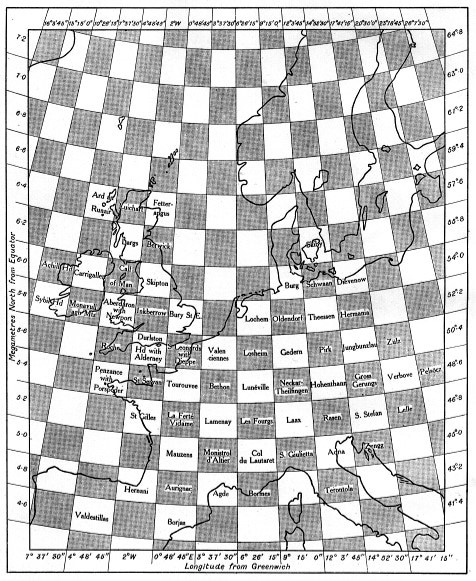
\includegraphics{eingeteilte_Karte.jpg}
	\caption{Gitter zur numerischen Approximation der Felder, welche das Wetter beeinflussen.
		Wie man sehen kann ist das Gitter sehr grob und somit ungenau.
		In der Schweiz, zum Beispiel hat es nur einen Gitterpunkt. 
		}
	\label{bild:karteEuropa}
\end{figure}

\begin{figure}
	\centering
	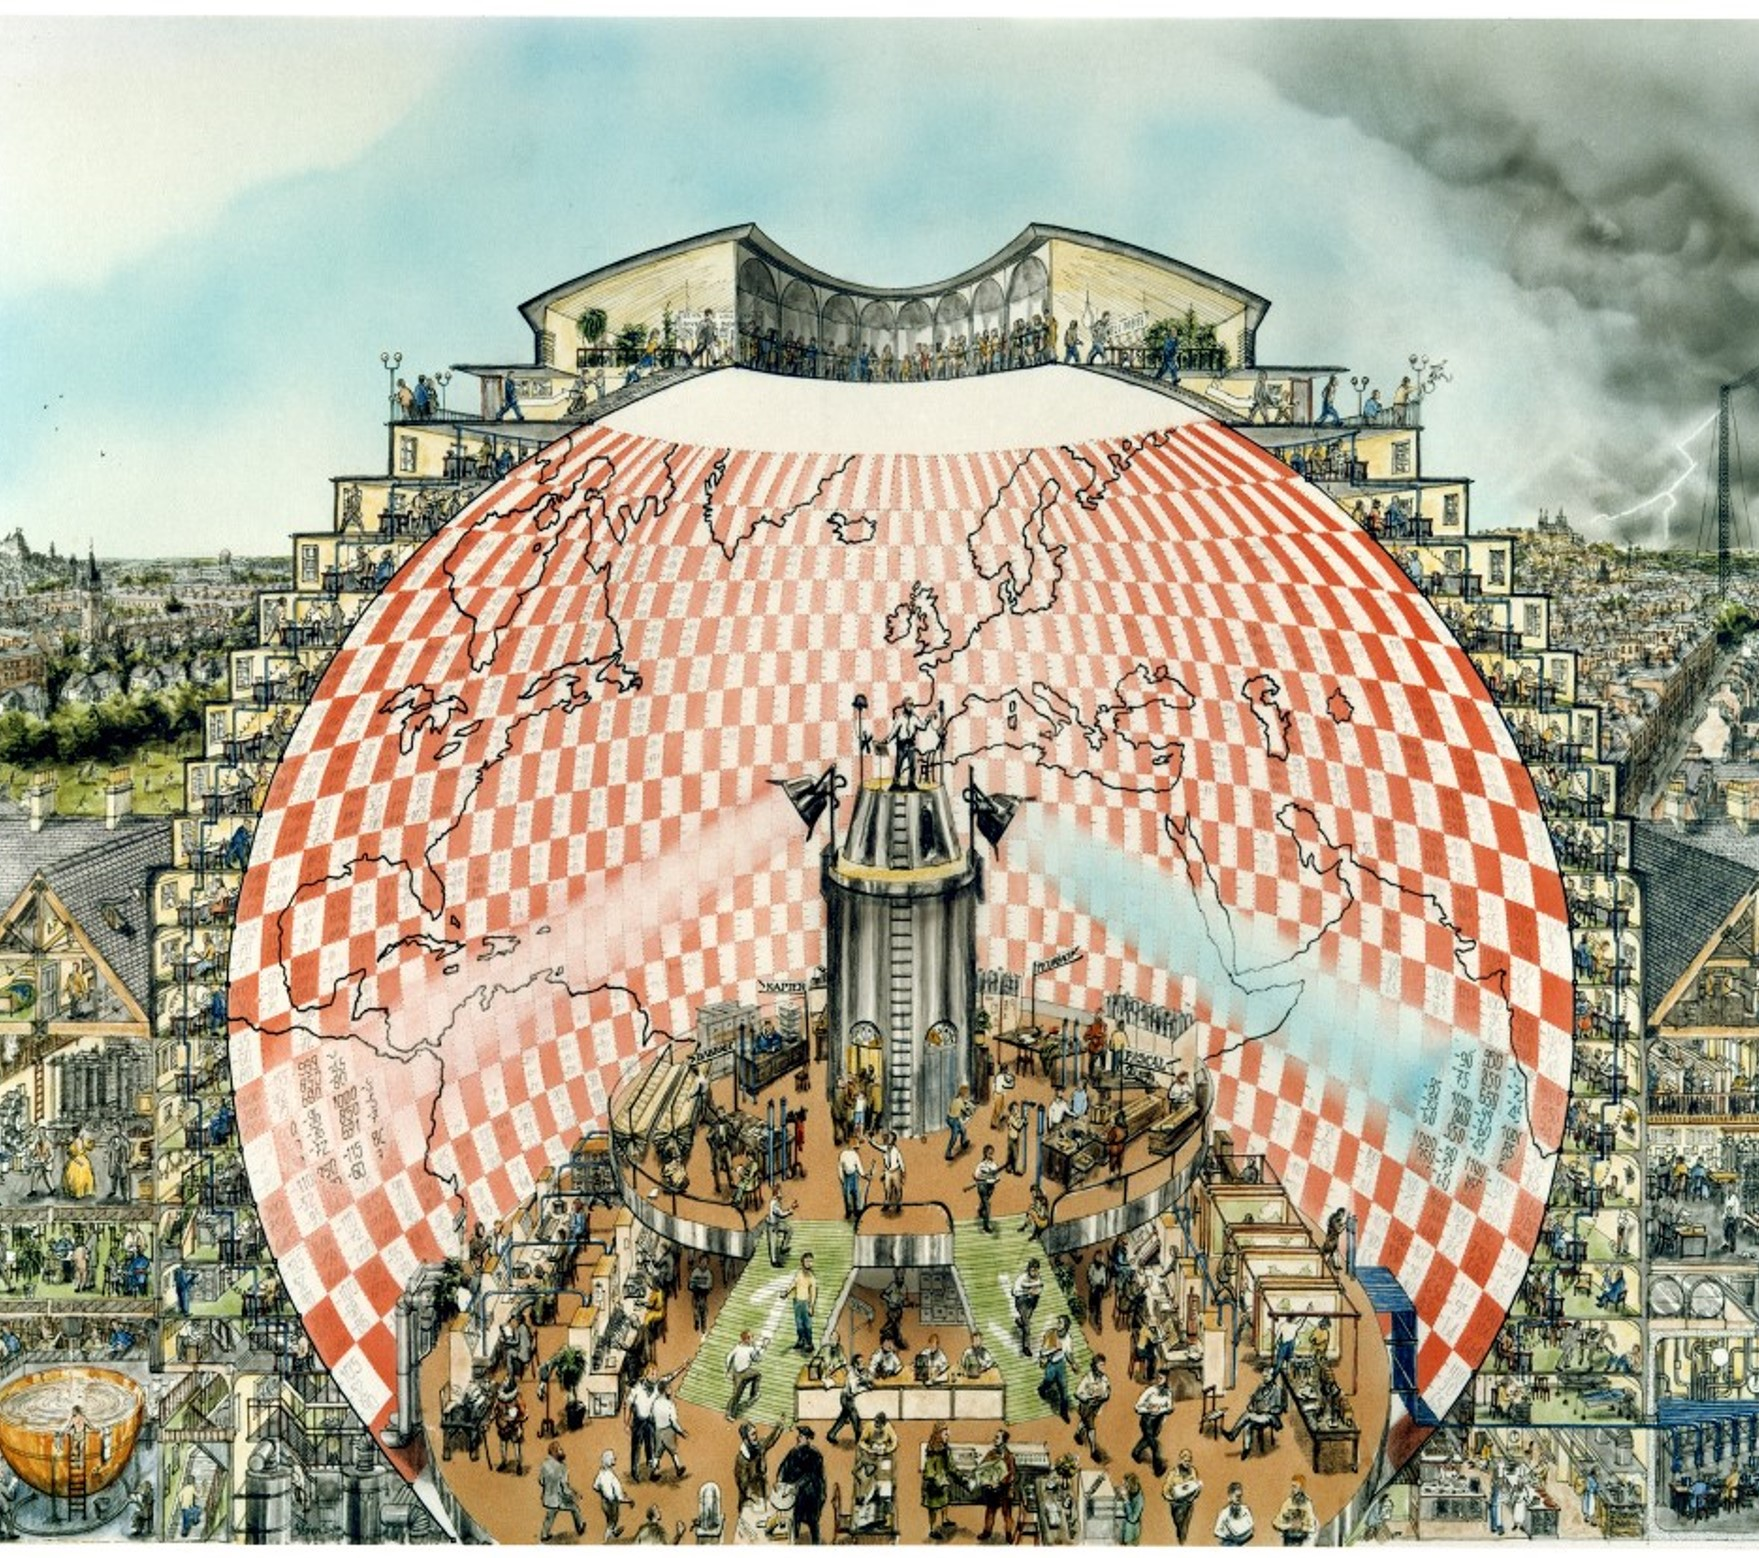
\includegraphics[width=\textwidth]{Richardsons_Traum.jpg}
	\caption{Traumvorstellung von Richardson einer Station zur Wettervorhersage. 
	Rundherum hängt eine Weltkarte und Leute berechnen ständig die Atmosphäre zu ihrem Bereich.}
	\label{bild:richardsonsTraum}
\end{figure}

\subsection{Grund der fehlerhaften Vorhersage \label{geostrophisch:subsection:failedPrediction}}

Trotz seines bahnbrechenden Ansatzes war Richardsons erste Wettervorhersage weit von der Realität entfernt. 
Sein Ergebnis sagte für den folgenden Tag einen Luftdruckanstieg von über \SI{145}{\hecto\pascal} voraus, was ein physikalisch völlig unrealistischer Wert ist. 
Weshalb war seine erste Vorhersage so falsch? 
Sein scheitern lag bestimmt nicht an mangelndem physikalischen Verständnis oder fehlerhafter Idee. 
Sondern es lag viel mehr an praktischen Problemen.
In der Atmosphäre kompensieren sich unter großräumigen Bedingungen normalerweise der Druckgradient und die Coriolis-Kraft näherungsweise, sodass sich ein nahezu stationärer, geostrophischer Wind einstellt.
Doch die Daten vom 20. Mai 1910, welche mittels den Wetterballonen aufgezeichnet wurden, befanden sich nicht im geostrophischen Gleichgewicht.
Grund dafür waren regionale Wetterstörungen wie Tiefdruckgebiete, Fronten und vertikale Strömungen, welche den idealisierten Ausgleich zwischen Druckgradient- und Coriolis-Kraft verhinderten.
Zudem wirkten in der unteren Troposphäre Reibungseinflüsse und kleinräumige Turbulenz, sodass Windgeschwindigkeit und -richtung deutlich von den geostrophischen Werten abwichen.
Die punktuell und zu unterschiedlichen Zeitpunkten erhobenen Messungen führten darüber hinaus zu inkonsistenten Druck- und Windfeldern.
Richardson setzte die Rohdaten – abgesehen von der Interpolierung auf das Gitter – unverändert in seine Bewegungsgleichungen ein, ohne zuvor eine Anpassung an das geostrophische Gleichgewicht vorzunehmen.
Dadurch traten in seiner Modellrechnung große Beschleunigungen auf, die schlussendlich zu seiner stark fehlerhaften Wettervorhersage führten.
Erst Jahrzehnte später wurde klar, dass für stabile numerische Prognosen ein Anfangszustand im geostrophischen Gleichgewicht oder zumindest nahe daran essentiell ist.


 



